%%%%%%%%%%%%%%%%%%%%%%%%%%%%%%%%%%%%%%%%%%%%%%%%%%%%%%%%%%%%
%%% LIVECOMS ARTICLE TEMPLATE
%%% ADAPTED FROM ELIFE ARTICLE TEMPLATE (8/10/2017)
%%%%%%%%%%%%%%%%%%%%%%%%%%%%%%%%%%%%%%%%%%%%%%%%%%%%%%%%%%%%
%%% PREAMBLE
\documentclass[9pt]{livecoms}
% Use the 'onehalfspacing' option for 1.5 line spacing
% Use the 'doublespacing' option for 2.0 line spacing
% use the 'lineno' option for adding line numbers.
% Please note that these options may affect formatting.

\usepackage[version=4]{mhchem}
\usepackage{siunitx}
\DeclareSIUnit\Molar{M}
\newcommand{\versionnumber}{1.0}  % you should update the minor version number in preprints and major version number of submissions.
%%%%%%%%%%%%%%%%%%%%%%%%%%%%%%%%%%%%%%%%%%%%%%%%%%%%%%%%%%%%
%%% ARTICLE SETUP
%%%%%%%%%%%%%%%%%%%%%%%%%%%%%%%%%%%%%%%%%%%%%%%%%%%%%%%%%%%%
\title{Best Practices for Quantification of Uncertainty and Sampling Quality in Molecular Simulations: v\versionnumber}

% Everyone should put in their name properly, institution, email
\author[1*\authfn{1}]{Alan Grossfield}
\author[2*\authfn{1}]{Pascal Merz}
\author[3*\authfn{1}]{Paul Patrone}
\author[4*\authfn{1}]{Daniel Roe}
\author[5*\authfn{1}]{Andrew Schultz}
\author[6*\authfn{1}]{Daniel Siderius}
\author[7*\authfn{1}]{Daniel M. Zuckerman}
\affil[1]{Institution 1}
\affil[7]{Oregon Health \& Science University}

\corr{email1@example.com}{FMS}  % Correspondence emails.  FMS and FS are the appropriate authors initials.
\corr{zuckermd@ohsu.edu}{DMZ}

\contrib[\authfn{1}]{These authors contributed equally to this work, we hope!}


%\presentadd[\authfn{3}]{Department, Institute, Country}
%\presentadd[\authfn{4}]{Department, Institute, Country}

%%%%%%%%%%%%%%%%%%%%%%%%%%%%%%%%%%%%%%%%%%%%%%%%%%%%%%%%%%%%
%%% ARTICLE START
%%%%%%%%%%%%%%%%%%%%%%%%%%%%%%%%%%%%%%%%%%%%%%%%%%%%%%%%%%%%

\begin{document}

\maketitle

\begin{abstract}
The quantitative assessment of uncertainty and sampling quality is essential in molecular simulation.
Many systems of interest are highly complex, at the edge the field's computational capacity, and it is important to understand and communicate statistical uncertainties so that `consumers' of the data understand the meaning and limitations of the simulation data.
This article covers key analyses appropriate for trajectory data straightforward simulation methods such as molecular dynamics and (single Markov chain) Monte Carlo, as well as providing guidance for analyzing some `enhanced' sampling approaches.
We do not discuss \emph{systematic} errors arising from inaccuracy in the chosen force field.
\end{abstract}

\section{Introduction: Scope and definitions}

\subsection{Scope}
This article is geared toward simulation studies attempting to quantify observables and derive reliable error bars based on `standard' canonical sampling methods (e.g., molecular dynamics and Monte Carlo) and associated “enhanced” sampling methods.  
Some problems and systems may be better studied with cruder techniques and analyses, which will not be covered here.
This article also will not cover issues of systematic error arising from inaccuracy in force field (underlying model) or even from the simulation setup.
Rather, this article will take raw trajectory data and face value, assuming it is a valid outcome given the underlying model.
We emphatically will \emph{not} assume that a trajectory has been sufficiently `equilibrated'.

\subsection{Key Definitions [to be refined]}
The reader should be familiar will a set of basic statistical and simulation concepts.
[and we should provide links/refs for each.]

\begin{itemize}
   \item Precision: The amount of variability in an estimate (based on repeating a given simulation protocol multiple times).  
      Better sampling in an individual simulation leads to higher precision.
    \item Accuracy: The degree of agreement with a reference value, which be an experimental measurement or the result of a well-sampled simulation.
    \item Raw data: The numbers that the computer program spits out as it runs
    \item Derived observables:  Quantities derived from ‘non-trivial’ analyses of raw data
\end{itemize}

\section{Best Practices Checklist}
\begin{enumerate}
\item
- Pre-simulation sanity checks and planning tips: There is no guarantee that any method (enhanced or otherwise) can sample any given system
    \begin{itemize}
    \item See best-practices papers on simulation background and planning/setup [Link out to simulation background and preparation documents - github]
    \item Are system timescales known experimentally and feasible computationally based on published literature?
    \item If timescales are too long for straight-ahead MD, is an enhanced method being used for which there are precedents for systems of similar complexity?
    \item Read a good article or book on sampling assessment (this one or a reference herein).  Understanding error is a technical endeavor.
    \item Key concept: Connection between the equilibrium ensemble and individual trajectory (may or may not reach equilibrium); equilibrium vs. non-equilibrium.
    \item Consider multiple runs vs. single run.  Multiple runs may be especially useful in assessing uncertainty for enhanced sampling methods.
    \item Make initial configuration as diverse as possible  … but note that if results depend on initial configs, that implies insufficient sampling (to be pedantic, it always does if sampling is finite, but it’s about figuring out variability and confidence intervals
    - Look for automated construction methods for reproducibility
    - Check your code/method via a simple benchmark system.  [Link out to software validation doc]
    \end{itemize}
\item
- Perform quick-and-dirty data checks which can rule out (but not ensure) sufficient sampling: Necessary vs. sufficient
    \begin{itemize}
    \item Look at time series -- think in advance about what states should exist. How many transitions do you see? If you have 1 transition, you can’t talk about populations
    \item Plot as many properties as you can think of, even if they’re not interesting
    \item Plot pairwise configurational distances (e.g., RMSD values for biomolecules) in greyscale for $\sim$100 evenly spaced frames
    \item Visualize the trajectory graphically -- look for slow motions.  BE SKEPTICAL!
    \item Compare observable different fractions of a run (DMZ thirds idea)
    \item Andrew: short vs. very short
    \item Daniel R: Compare runs from different initial conditions - be sure initial conditions are ‘different enough’
    \end{itemize}    
\item
- Remove an ‘equilibration’/’burn in’/transient portion of a single MD or MC trajectory and perform analyses only on remaining ‘production’ portion of trajectory.
\item
- Consider computing a quantitative measure of global sampling [biomolecular vs. materials problems] - i.e., how many statistically independent samples do you have?
\item
- Quantifying error in specific observables of interest [general approaches]
    - Key concept: Difference between between scale of variation (measured by variance) and statistical uncertainty
\item
- If you’re using an enhanced sampling method, …
    - Key concept: Complexity of correlations in advanced methods
\end{enumerate}

% !TEX root = ./main.tex

\section{Quick-and-Dirty checks that can rule out good sampling}
\label{sec:quick}

It is difficult to establish with certainty that good sampling has been achieved, but it is not difficult to \emph{rule out} high-quality sampling.
Here we elaborate on some quick-and-dirty tests that quickly show inadequacies in sampling.

\subsection{Zeroth-order system-wide tests}

The simplest test for poor sampling is lack of equilibration: if the system is still noticeably relaxing from its starting conformation, statistical sampling has not even begun, and thus by definition is poor.  As a result, the very first test should be to verify that the basic equilibration has occurred.  To check for this, one should inspect the time series for a number of simple scalar values, such as potential energy, system size (and area, if you are simulating a membrane or other system where one dimension is distinct from the others), temperature (if you are simulating in the NVE ensemble), and/or density (if simulating in the isothermal-isobaric ensemble).  Often, simple visual inspection is sufficient to determine that the simulation is systematically changing, although more sophisticated methods have been proposed by Chodera \cite{Chodera-2016}.  If \emph{any} value appears to be systematically changing, then the system is not equilibrated.

\subsection{Tests based on configurational distance measures - e.g., RMSD for biomolecules}

\begin{wrapfigure}{r}{6cm}
  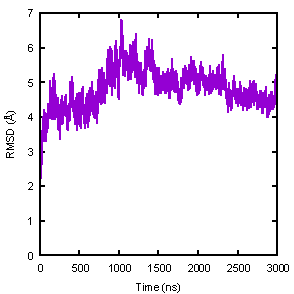
\includegraphics[width=5.8cm]{figures/rmsd/rmsd}
  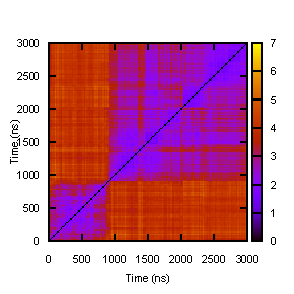
\includegraphics[width=5.8cm]{figures/rmsd/rmsds}
  \caption{
  \label{f:rmsd} RMSD as a measure of convergence.  The upper panel shows the
  $\alpha$-carbon RMSD of the protein rhodopsin from its starting structure as a
  function of time.  The lower panel shows the all-to-all RMSD map computed from the same
  trajectory.  Data from Leioatts, et al \cite{Grossfield-2015}.
  }
\end{wrapfigure}

We will use the standard biomolecular RMSD (root mean-squared difference) as a generic distance measure for illustrative purposes.
Alternatives to RMSD could be a dihedral-angle distance or another measure specific to your system of interest.
Note that RMSD, like any distance in a high-dimensional space, becomes ``degenerate'' for larger values: given a reference configuration, there are a large number of configurations which differ from the reference by a given large RMSD. This is analogous to the increasing number of points in three-dimensional space with increasing radial distance from a reference point, except much worse because of the dimensionality. For a detailed exploration of expected RMSD distributions for biomolecular systems see the work of Pitera.\citep{Pitera2014}

Some qualitative tools for assessing global sampling based on RMSD were reviewed
in prior work \cite{Grossfield2009}.   The classic time series plot of RMSD with
respect to a crystal or other single reference structure can immediately
indicate whether the structure is still systematically changing.  Although this
kind of plot was historically used as a sampling test, it should really be
considered as another equilibration test like those discussed above.  Moreover,
it's not even a particularly good test of equilibration, because the degeneracy
of RMSD means you can't tell if the simulation is exploring new states that are
equidistant from the chosen reference.  The upper panel of Figure \ref{f:rmsd}
shows a typical curve of this sort, taken from a simulation of the G
protein-coupled receptor rhodopsin \cite{Grossfield-2015}; the curve increases
rapidly over the few nanoseconds and then roughly plateaus.  It is difficult to
assign meaning to the other features on the curve.

A better RMSD-based convergence measure is the all-to-all RMSD plot; taking the
RMSD of each snapshot in the trajectory with respect to all others allows you to
use RMSD for what it does best, identifying very similar structures.  The lower
panel of Figure \ref{f:rmsd} shows an example of this kind of plot, applied to
the same trajectory before.  By definition, all such plots have values of zero
along the diagonal, and occupation of a given state shows up as a block of
similar RMSD along the diagonal; in this case, there are 2 main states, with one
transition occuring roughly 800 ns into the trajectory.  Off diagonal ``peaks''
(regions of low RMSD between structures sampled far apart in time) indicate that
the system is revisiting previously sampled states, a necessary condition for
good statistics.  In this case, the initial state is never sampled after the
first transition, but there are a number of small transitions within the second
state.

\subsection{Assessing Convergence}
Convergence in the context of biomolecular simulations typically refers to the overlap of two independent measurements of the same property. If a measure is not converged it is a strong indication that sampling is poor. There are two common ways to try to obtain independent measurements. Arguably the best way is to have multiple independent simulations, each with varying initial starting conditions. Ideally these starting conditions should in some way span the space to be sampled; this way one can have confidence that simulations are not being trapped in a local minimum. For example, say the goal is to sample the phi and psi torsions of alanine dipeptide: the phi and psi angles for one simulation could be started from an alpha-helical conformation, while another simulation could be started from a polyproline II conformation. It is important to note that the starting conditions only need to be varied enough so that the desired space is sampled. For example, if the goal is to sample protein folding and unfolding, there should be some simulations started from the folded conformation and some from the unfolded, but if it is not important to consider protein folding no initial conformation needs to be unfolded.

Another way to obtain independent measurements is to divide a single simulation into two or more subsets. However this can at times be problematic because it can be more difficult to tell if the system is trapped in a local minimum since there is a single starting point. Those employing this approach should take extra care to assess their results (see in particular sections on 'block averaging' below).

There are two simple ways to compare independent measurements of a property. The simplest is to compare the arithmetic means and standard deviations. If these values do not overlap then convergence has not been achieved. However, since this assumes that the values are normally distributed, a better way is compare the overlap of the probability distributions (i.e. the histograms). This can be done via Kullback-Leibler or Jensen-Shannon divergence.
\section{Quantification of Global Sampling}
\label{sec:global}


With ideal trajectory data, one would hope to be able to compute arbitrary observables with reasonably small error bars.
During a simulation, it is not uncommon to monitor specific observables of interest, but after the data are obtained, it may prove necessary to compute observables not previously considered.
These points motivate the task of estimating global sampling quality, which can be framed most simply in the context of single-trajectory data:
``Among the very large number of simulation frames (snapshots), how many are statistically independent?''
This number is called the \emph{effective sample size.}
From a dynamical perspective evoking auto-correlation ideas, which also apply to Monte Carlo data, how long must one wait before the system completely loses memory of its prior configuration?
The methods noted in this section build on ideas already presented in Sec.\ \ref{sec:quick} on qualitative sampling analysis, but attempt to go a step further to quantify sampling quality.

We emphasize that \emph{no single method described here has emerged as a clear best practice.}
However, because the global assessment methods provide a powerful window into overall sampling quality, which could easily be masked in the analysis of single observables (Sec.\ \ref{sec:specific}), we strongly encourage their use.
The reader is encouraged to try one or more of the approaches in order to understand the limitations of their data.


A key caveat is needed before proceeding.
Analysis of trajectory data generally cannot make inferences about parts of configuration space not visited \cite{Grossfield2009}.
It is generally impossible to know whether configurational states absent from a trajectory are appropriately absent because they are highly improbable (extremely high energy) or because the simulation simply failed to visit them because of a high barrier or random chance.

\subsection{Global sampling assessment for a single trajectory}
Two methods applicable for a single trajectory were previously introduced by some of the present authors, exploiting the fact that trajectories typically are correlated in time.
That is, each configuration evolves from and is most similar to the immediately preceding configuration;
this picture holds for standard MD and Markov-chain MC.
Both analysis methods are implemented as part of the software package LOOS \cite{LOOS,LOOS-JCC}.

\begin{figure}
  \centering
  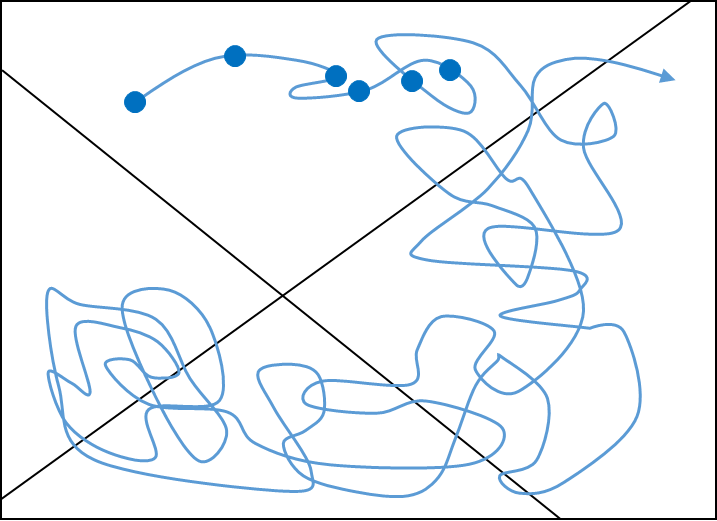
\includegraphics[width=0.8\linewidth]{decorr-graphic.png}
  \caption{The basis for ``decorrelation analysis'' \cite{Lyman2007a}.
  From a continuous trajectory (blue curve), configurations can be extracted at equally spaced time points (filled circles) with each such configuration categorized as belonging to one of a set of arbitrary states (delineated by straight black lines).  
  If the configurations are statistically independent -- if they are sufficiently decorrelated -- then their statistical behavior will match that predicted by a multinomial distribution consistent with the trajectory's fractional populations in each state.
  A range of time-spacings can be analyzed to determined if and when such independence occurs.}
  \label{fig:decorr}
\end{figure}

Lyman and Zuckerman proposed a global ``decorrelation'' analysis by mapping a trajectory to a discretization of configuration space (set of all $x, y, z$ coordinates) and analyzing the resulting statistics \cite{Lyman2007a}.
Configuration space is discretized into bins based on Voronoi cells of structurally similar configurations,  e.g., using RMSD defined in Eq.\ \ref{eq:rmsd} or another configurational similarity measure; reference configurations for the Voronoi binning are chosen at random or more systematically as described in \cite{Lyman2007a}.
Once configuration space is discretized, the trajectory frames can be classified accordingly, leading to a discrete (i.e., 'multinomial') distribution (Fig.\ \ref{fig:decorr}).
The analysis method is based on the observation that the variance for any bin of a multinomial distribution is known, given the bin populations (from trajectory counts) and a specified number of independent samples drawn from the distribution \cite{Lyman2007a}.
The knowledge of the expected variance allows testing of increasing waiting times between configurations drawn from the trajectory to determine when and if the variance approaches that expected for independent samples.
The minimum waiting time yielding agreement with ideal (i.e., uncorrelated) statistics yields an estimate for the decorrelation/memory time, which in turns implies an overall effective sample size. 



A second method, employing block covariance analysis (BCOM), was presented by Romo and Grossfield \cite{Romo2011} building on ideas by Hess \cite{Hess2002}.  In essence, the method combines two standard error analysis techniques --- block averaging \cite{Flyvbjerg-1989} and bootstrapping \cite{Tibshirani1998} --- with covariance overlap, which quantitatively measures the similarity of modes determined from principal component analysis (PCA) \cite{Hess2002}.  PCA in essence generates a new coordinate system for representing the fluctuation in the system while tracking the importance of each vector; the central idea of the method is to exploit the fact that as sampling improves, the modes generated by PCA should become more similar, and the covariance overlap will approach unity in the limit of infinite sampling.

When applying BCOM, the principal components are computed from subsets of the trajectory, and the similarity of the modes evaluated as a function of subset size; as the subsets get larger, the resulting modes become more similar.  This is done both for contiguous blocks of trajectory data (block averaging), and again for randomly chosen subsets of trajectory frames (bootstrapping); taking the ratio of the two values as a function of block size yields the degree of correlation in the data.  Fitting that ratio to a sum of exponentials allows one to extract the relaxation times in the sampling.  The key advantage of this method over others is that it implicitly takes into account the number of substates; the longest correlation time is the time required not to make a transition, but to sample a scattering of the relevant states. 

\subsection{Global sampling assessment for multiple independent trajectories}
\label{sec:globalMultiTraj}
When sampling is performed using multiple independent trajectories (whether MD or MC), additional care is required.
Analyses based solely on the assumption of sequential correlations may break down because of the unknown relationship between separate trajectories.

Zhang et al.\ extended the decorrelation/variance analysis noted above, while still retaining the basic strategy of inferring sample size based on variance \cite{Zhang2010}.
To enable assessment of multiple trajectories, the new approach focused on conformational state populations, arguing that the states fundamentally underlie equilibrium observables.
Here, a state is defined as a finite region of configuration space, which ideally consists of configurations among which transitions are faster than transitions among states; 
in practice, such states can be approximated based on kinetic-clustering Voronoi cells according to the inter-state transition times \cite{Zhang2010}.
Once states are defined, the approach then uses the variances in state populations among trajectories to estimate the effective sample size, motivated by the decorrelation approach \cite{Lyman2007a} described above.

Nemec and Hoffmann proposed related sampling measures geared specifically for analyzing and comparing multiple trajectories \cite{Nemec2017}.
These measures again do not require user input of specific observables but only a measure of the difference between conformations, which was taken to the be the RMSD.
Nemec and Hoffmann provide formulas for quantifying the conformational overlap among trajectories (addressing whether the same configurational states were sampled) and the density agreement (addressing whether conformational regions were  sampled with equal probabilities).




\section{Computing error in specific observables}
- Basics: how to report, what goal to shoot for, significant figures
- When should you not trust uncertainties
    - Unknown unknowns
- If calculating a derived quantity, consider error in conversion from raw data 
    - Propagation of error (this doesn’t mean publishing your results!)
    - Taylor series expansion can handle cases where derived quantity is a direct function of measured data
    - Wikipedia: Propagation of uncertainty
    - Generate synthetic data with noise model [Paul]
    - Data filtering [Paul]
    - Bootstrapping [Andrew/Dan S]
used for cases where the derived quantity is not simple function of the measured data.
An Introduction to the Bootstrap
    - Need to know correlation to correctly estimate sample size
    - Otherwise just gives relative uncertainty
- Correlation time analysis [Dan Z]
- Block averaging [Dan Z/Alan?/Dan S] Flyvjberg and Petersen 
- ‘Dark uncertainty’ analysis [Paul]
- MOST OF THESE ALGORITHMS FAIL IF THE TRAJECTORY IS WAY TOO SHORT
    - If you miss the timescale by enough, you can’t tell
    - YOU HAVE TO THINK ABOUT THIS IN ADVANCE
- Link out to transport doc

\section{Enhanced sampling [Write as supplements, which can later be broken out as separate documents?]}
- Compare to standard sampling (e.g., straight MD) for a simple system
- Complex correlation structures in complex methods indicate comparison of multiple independent runs will be useful
    - Explain what to compare [Dan Z]
- Replica exchange [Daniel Roe]
    - Round-trips (necessary but not sufficient)
    - Compare ‘coordinate trajectories’ - distributions from temperature/Hamiltonian-wandering trajectories should match
    - Examine replica residence times
- Weighted ensemble (WE)
    - See this WE overview doc, particularly limitations section
    - Key concept: ‘Tree’ of trajectories generated by WE leads to strong correlations, requiring care
    - Key concept: WE simulation generically relaxes from the initial distribution toward the ultimate distribution which could be equilibrium (if no feedback/recycling or external driving) or a non-equilibrium steady state (if feedback from specified target to initial state)
    - Safest approach: Use multiple runs, which are fully independent.  Perform as many runs as needed to reduce the statistical uncertainty (std err of mean) for quantity of interest
    - For a single observable, the time course of the value can be analyzed using the usual methods of analyzing time-correlated data (see above - e.g., block-averaging)


% we will have a bunch of includes here


\section{Acknowledgments}

Funder and other information can be given here.

\bibliography{refs}
\bibliographystyle{vancouver-livecoms}

\end{document}
